\documentclass[10pt]{article}
\usepackage[margin=1.2in]{geometry}

%\usepackage{algpseudocode}
%\usepackage{algorithm}

\usepackage[utf8]{inputenc}
\usepackage[ngerman]{babel}

\usepackage{graphicx}
\usepackage{fmtcount}

\usepackage{multirow}

\usepackage[hyphens]{url}
\usepackage{hyperref}

\usepackage{array}
\usepackage{amsmath}
\usepackage{amssymb}

%\usepackage{natbib}

\usepackage{mathtools}

\usepackage{listings}
\usepackage{color}
\usepackage{booktabs}

% keywords: fixme

\sloppy

\begin{document}

\title{Effiziente Methoden für die Bit-Reversed Permutation in 
	{\tt C++11} auf der x86-64 Architektur }

\author{Christian Knauth\\
Freie Universit\"at Berlin\\
Institut f\"{u}r Informatik
\and
Boran Adas\\
Freie Universit\"at Berlin\\
Institut f\"{u}r Informatik
\and
Daniel Whitfield\\
Freie Universit\"at Berlin\\
Institut f\"{u}r Informatik
\and
Xuesong Wang\\
Freie Universit\"at Berlin\\
Institut f\"{u}r Informatik
\and
Lydia Ickler\\
Freie Universit\"at Berlin\\
Institut f\"{u}r Informatik
\and
Tim Conrad\\
Freie Universit\"at Berlin\\
Institut f\"{u}r Informatik
\and
Oliver Serang\\
Freie Universit\"at Berlin\\
Institut f\"{u}r Informatik\\
\url{orserang@uw.edu}
}

\date{{\small \today}}

\maketitle

\begin{abstract}
\noindent Die {\it Bit-Reversed Permutation} ist eine wichtige Methode 
in der Signalverarbeitung und der Schlüssel zur effektiven Implementierung der 
{\it Schnellen Fourier-Transformation}. Diese Arbeit präsentiert 
optimierte Implementierungen in {\tt C++} fünf bereits existierender Methoden 
zur Berechnung der Bit-Reversed Permutation:
{\it Stockham Auto-Sort}, {\it Naive Bitwise Swapping}, Vertauschung (Swapping) mittels 
einer Tabelle reverser Bytes, lokales paarweises Swapping von Bits sowie Swapping 
mittels eines cachelokalen Matrix-Buffers. Drei neue Strategien, die Bit-Reversed 
Permutation durchzuführen werden vorgestellt: 
Eine induktive Methode unter Nuzung der Bitoperation XOR, eine {\it template-rekursive}
geschlossene Form ({\it Unrolled Methode}), sowie einen {\it cache-oblivious}, template-rekursiven Ansatz, 
welcher das Ausgangsproblem auf kleinere Bit-Reversed Permutations, 
sowie die Transposition einer quadratischen Matrix reduziert. 
Diese neuen Methoden werden mit den existenten Ansätzen bzgl. der theoretischen Laufzeit, 
empirischen Kompilerdauer, sowie empirischen Laufzeit verglichen. Es wird gezeigt, dass 
die template-rekursive Methode mit den schnellsten bisher bekannten Ansätzen 
konkurrieren kann, allerdings leichter von einer Parallelisierung auf mehreren CPU-Cores
aber auch der GPU profitieren kann.
\end{abstract}

\section*{Einleitung}
Die klassische schnelle Fourier Transformation (FFT) nach Cooley und Tukey 
reduziert das Ausgangsproblem rekursiv auf zwei FFTs der halben Größe (eine wertet die 
geradzahligen Indizes aus, die andere die ungeradzahligen) \cite{cooley:algorithm}. 

Das Cooley-Tukey Verfahren ist sehr wichtig durch seine vielen Anwendungen im Bereich des 
wissenschaftlichen Rechnens: Beispielsweise erlaubt die FFT die numerische Berechnung der 
Konvolution, oder Faltung, zweier Arrays der Länge $n$ in $O(n \log(n))$ Schritten, anstelle von 
$O(n^2)$ Schritten, wie sie für den naiven Konvolutionsalgorithmus benötigt würden.\cite{proakis:introduction}. 
Die Einfachheit, Effizienz und vielseitige Nützlichkeit Cooleys und Tukeys Arbeit hat dazu geführt, 
dass diese heute als eine der einflussreichsten informatischen Methoden des \ordinalnum{20} 
Jahrhunderts angesehen wird.\cite{cipra:best}.

Der einfachste Weg die Cooley-Tukey FFT zu berechnen ist {\it out-of-place} unter 
Benutzung eines Buffers der Größe $n$. Dann können die Werte aus dem ursprünglichen Array in andere 
Positionen des Buffers kopiert werden, sodass die geradzahligen Indizes des Arrays nun die Indizes $0, 1, \ldots
\frac{n}{2}-1$ des Buffers einnehmen und die ungeradzahligen Indizes des Arrays dementsprechend die 
Stellen $\frac{n}{2}, \frac{n}{2}+1, \ldots n-1$ des Buffers einnehmen.
Dieser Ansatz wird gemeinhin als ``Stockham Auto-Sort''\cite{cochran:fast} bezeichnet.

Die FFT {\it in-place} zu Berechnen (also das Eingabearray zu überschreiben, 
ohne dass ein Buffer für die Ergebnisse benötigt wird) ist jedoch anspruchsvoller.
Die {\it Even-Odd-Permutation}, also die schrittweise Vertauschung geradzahliger mit ungeradzahligen Indizes, 
wie sie bei der Stockham-FFT durchgeführt wird, ist äquivalent zu einer $\frac{n}{2} \times 2$ 
Matrix-Transposition. Wäre beispielsweise $n=8$, können die Indizes $[0, 1, 2, 3, 4, 5, 6, 7]$ 
als $4 \times 2$ Matrix begriffen werden, deren Transposition dann der gewünschten Even-Odd-Permutation entspricht:
\[ 
\left[
  \begin{matrix}
    0 & 1\\
    2 & 3\\
    4 & 5\\
    6 & 7
  \end{matrix}
\right]^T = 
\left[
  \begin{matrix}
    0 & 2 & 4 & 6\\
    1 & 3 & 5 & 7
  \end{matrix}
\right],
\]

wobei sich die Werte an geradzahligen Index-Positionen nun in der ersten Reihe, 
die Werte an ungeradzahligen Index-Positionen in der zweiten Reihe befinden.
Diese Transposition ist die Inverse des sog. ``Faro-Shuffle'', oder auch ``Perfect-Shuffle''\cite{sedgewick:algorithms}, 
bei dem ein Karten-Deck geteilt wird und beide Hälften verzahnt und dann ineinander geschoben werden.
Eine in-place FFT erfordert, dass diese Matrix-Transpositionen ebenfalls in-place durchgeführt werden, 
d.h. sie deutlich weniger als $n$ zusätzlichen Speicher benötigen. In-place Transposition von nicht quadratischen Matritzen
ist jedoch anspruchsvoll, denn der Wert an der Zielposition, in die geschrieben wird, wird nicht notwendigerweise mit 
dem Wert an der Ausgangsposition vertauscht, wie es bei einer quadratischen Matrix der Fall wäre.
Um eine $M \times N$ Matrix zu transponieren, wobei höchstens $O(M + N)$ an Speicher genutzt wird, benötigen 
existierende Algorithmen eine Laufzeit  $\in \Omega(M N \log(M N))$\cite{fich:permuting}.

Aber selbst wenn ein schneller $O(n)$ Algorithmus for die Even-Odd-Permutation verfügbar wäre, 
und dieser nicht signifikant zusätzlichen Speicher benötigen würde (möglicherweise unter 
Ausnutzung der Eigenschaft, dass es sich um einen Spezialfall der Matrix-Transposition handelt), 
trennt diese Permutation die FFT der Länge $n$ von den rekursiven FFTs der Länge $\frac{n}{2}$, 
was einen negativen Effekt haben kann, indem es den Compiler daran hindert, gemeinsamen Code in den rekursiven 
Methodenaufrufen zu erkennen, wie beispielsweise wiederverwendete trigonometrische Konstanten.
FFT-Code, der Compiler-Optimierung ermöglicht, ist hoch geschätzt \cite{myrnyy:simple}.

Ein Ansatz ist es, alle Even-Odd-Permutationen zu Beginn der FFT durchzuführen. 
Jede Even-Odd-Permutation kann auch als Vertauschung des am wenigsten signifikanten 
Bits mit dem signifikantesten Bit begriffen werden; eine sequentielle Ausführung aller 
Even-Odd-Permutationen ist daher äquivalent dazu, alle 
Indizes mit den Indizes zu Vertauschen, die mit ihren umgekehrten Bit-Strings korrespondieren. 
Die ``Bit-Reversed Permutation'' von  $[0, 1, 2, 3, 4, 5, 6, 7]$, oder $[000,
  001, 010, 011, 100, 101, 110, 111]$ in binärer Schreibweise, wäre $[0, 4, 2,
  6, 1, 5, 3, 7]$, oder eben $[000, 100, 010, 110, 001, 101, 011, 111]$. 
  Gegeben eine Funktion {\tt rev}, die Indizes bitweise umkehrt, lässt sich die 
Bit-Reversed Permutation ziemlich unkompliziert durchführen({\bf
Listing~\ref{alg:simple-permutation}}). Man beachte, dass die Bit-Reversed 
Permutation in-place durchgeführt werden kann, indem einfach die Werte korrespondierender 
Paare von Index und reversem Index vertauscht werden, was weniger kompliziert ist, als eine 
in-place Matrix-Transposition einer nicht-quadratischen Matrix, da die Garantie 
{\tt rev(rev(i)) = i} gilt (in gewisser Weise ähnlich der Transposition einer 
quadratischen Matrix).

Nach Anwendung einer Bit-Reversed Permutation kann die FFT dann einfach durch eine geringfügig 
modifizierte Version des Algorithmus durchgeführt werden, bei der nun angenommen werden kann, 
dass in jeder Stufe der Rekursion bereits eine Even-Odd-Permutation stattgefunden hat.

\begin{footnotesize}
  \lstset{language=C++,
    basicstyle=\ttfamily,
    keywordstyle=\color{blue}\ttfamily,
    stringstyle=\color{red}\ttfamily,
    commentstyle=\color{magenta}\ttfamily,
    morecomment=[l][\color{magenta}]{\#},
    breaklines=true,
  }
\begin{lstlisting}[label={alg:simple-permutation},
caption={
%fixme
{\bf Durchführung einer Bit-Reversed Permutation mithilfe einer externen {\tt rev}-Funktion. } 
Sei {\tt LOG\_N} die Problemgröße spezifiziert als {\tt constexpr} (\emph{d.h.}, {\tt LOG\_N} ist zur Kompilierzeit 
als Konstante bekannt). Man Beachte, dass die Funktion {\tt rev} ein Template abhängig von der Problemgröße ist.}]
void naive_bitwise_permutation(T*__ restrict const v) {
  constexpr unsigned long int N = 1ul << LOG_N;

  for (unsigned long index=1; index<(N-1); ++index) {
    unsigned long reversed = rev<LOG_N>(index);

    // Comparison ensures swap is performed only once per unique pair (otherwise, every index will be swapped and then swapped back to re-create the original array):
    if (index<reversed)
      std::swap(v[index], v[reversed]);
  }
}
\end{lstlisting}
\end{footnotesize}

Obwohl einige Digital-Signal-Prozessoren (DSPs) native {\it Bit-Reversal} 
Operationen unterstützen, fehlt es vielen modernen Desktop-CPUs 
(einschließlich der {\tt x64}-Architektur) an entsprechendem Opcode; weshalb
effiziente Funktionen um {\tt rev} zu berechnen notwendig sind.

Selbstverständlich kann Bit-Reversal bitweise in $\Theta(b)$, wobei $n = 2^b$ und $b$ {\tt
  LOG\_N} im {\tt C++}-Code entspricht, durchgeführt werden. Die Durchführung der vollen Bit-Reversed
Permutation mittels dieser naiven Bit-Reversal Methode benötigt daher
$\Theta(n b) = \Theta(n \log(n))$ Schritte.

\paragraph{Bytewise bit reversal:}
% fixme consistent Heading/Name style

Da die Bit-Reversal Funktion {\tt rev } an jeder Indexposition aufgerufen wird,
kann es von Vorteil für die Performanz sein, sie zu optimieren. Eine Möglichkeit, 
das Bit-Reversal signifikant schneller als mit dem naiven Ansatz durchzuführen ist es, 
ganze Blocks der Größe 1 Byte zu {\it swappen}\footnote{swappen meint das Vertauschen zweier Einträge im Speicher}, 
als nur einzelne Bits. Das wird effizient erreicht,
indem ein Array von {\tt unsigned-char}s mit 256 Einträgen, also einen Eintrag für jedes mögliche Byte,
vorberechnet wird. Für jedes Byte {\tt B} gibt ein Zugriff auf die Tabelle an Position {\tt B} das reverse Bit
von {\tt b} zurück. \cite{j:best,anderson:bit}. 
% fixme checke Swapping
Mit dieser Tabelle von reversen Bytes kann der selbe Ansatz wie beim Naive-Bitwise Swapping
verwendet werden. Dieser benötigt $\frac{b}{8}$ anstatt $b$ Schritte, wie die Naive-Bitwise Methode.
Die Bytewise Methode ist in der Praxis sehr viel schneller, obwohl ihre asymptotische Laufzeit, 
ebenso wie die der Naiv-Bitwise Methode weiterhin in $\Theta(n\log(n))$ liegt.

Jedoch, selbst wenn die Bit-Reversal Funktion {\tt rev} nativ unterstützt werden 
und in $O(1)$ CPU-Taktzyklus laufen würde, so sind die nicht-sequentiellen Speicherzugriffe
im hierarchischen Standard-Speichermodell (das zusammenhängende Speicherbereiche in den Cache lädt, 
jedes Mal wenn ein Wert benötigt wird der sich nicht im Cache befindet), das von {\tt x64} Computern 
verwendet wird, sehr ineffektiv. Dies steht im Gegensatz zu dem restlichen FFT-Code, dessen Speicherzugriffe 
in beinahe perfekt sequentieller Ordnung ablaufen (und der daher sehr effektiv bzgl. der 
Chache-Performance ist). Eine Folge davon ist, dass die Berechnung einer großen FFT einen signifikanten
Anteil ihrer Laufzeit in der Bit-Reversed Permutation verbringt.

% segue into pairwise bit reversal method
\paragraph{Bitweise Umkehrung mit Paaren von Bits:}
%fixme heading,

Eine Methode die Chache-Performance zu verbessern arbeitet zwar bitweise, 
verarbeitet jedoch immer zwei Bits in einem Schritt, indem immer das signifikanteste mit 
dem insignifikantesten Bit vertauscht wird.
Die Swaps werden, anstatt den kompletten reversen Index zu berechnen und zu swappen, wenn {\tt index < rev(index)}
nach jeder Vertauschung ausgeführt. Es wird also eine größere Anzahl von Swaps ausgeführt, die allerdings 
eine bessere Lokalität haben. Obwohl die Speicherzugriffe nicht in sequentiell angeordneten Blöcken erfolgen, 
liegen diese näher beieinander als bei der naiven und der Bytewise Methode. Trotz der größeren Anzahl von 
Swap-Operationen ist die asymptotische Laufzeit dieses Ansatzes die selbe wie die des Naiven, 
liegt also in $\Theta(n \log(n))$.

\paragraph{Bit-Reversal unter Nutzung eines Matrix Buffers:}
Carter \& Gatlin haben eine cache-optimierte Methode unter Nutzung eines Matrix-Buffers
vorgeschlagen. Die prinzipielle Idee ist, dass der Buffer klein genug ist um komplett in den 
{\tt L1} oder {\tt L2} Cache zu passen, der Buffer also Zeilenweise oder Spaltenweise durchlaufen 
werden kann und dennoch eine gute Cache-Performance erreicht. Gegeben {\tt index = x y z}, wobei die Bitstrings
{\tt x} und {\tt z} die gleiche Größe $\log(\sqrt{t})$ haben, wird ein Matrix-Buffer der Größe 
$\sqrt{t} \times \sqrt{t} = t$ verwendet \cite{carter:towards}.

% fixme checke out-of-place
Da {\tt rev(index) = rev(z) rev(y) rev(x)} gilt, würde eine out-of-place Methode für die Bit-Reversed Permutation
$\forall$~{\tt x},~$\forall$~{\tt y},~$\forall$~{\tt z},~{\tt
  dest[rev(z)~rev(y)~rev(x)]~$\gets$~source[x~y~z]} kopieren. 
Diese Methode, COBRA genannt \cite{carter:towards}, führt zwei Schritte aus: 
\noindent $\forall$~{\tt y},\\
\mbox{} \quad $\forall$~{\tt x},~$\forall$~{\tt z},~{\tt
  buff[rev(x)~rev(z)]~$\gets$~source[x~y~z]}\\
\mbox{} \quad $\forall$~{\tt x},~$\forall$~{\tt z},~{\tt
  dest[z~rev(y)~x]~$\gets$~buff[x~z]}.\\

\noindent Diese können geringfügig modifiziert werden zu:

\noindent $\forall$~{\tt y},\\
\mbox{} \quad $\forall$~{\tt x},~$\forall$~{\tt z},~{\tt
  buff[rev(x)~z]~$\gets$~source[x~y~z]}\\
\mbox{} \quad $\forall$~{\tt x},~$\forall$~{\tt z},~{\tt
  dest[rev(z)~rev(y)~x]~$\gets$~buff[x~z]}.\\

Obwohl Carter \& Gatlin eine out-of-place Implementierung (d.h. es wird nach {\tt dest} 
geschrieben anstatt {\tt source} zu modifizieren) beschreiben, ist es möglich
diese auch als In-Place-Verfahren zu adaptieren, bei der Swaps auf {\tt buff} 
durchgeführt werden, anstatt aus {\tt buff} oder nach {\tt buff} zu kopieren.  
Dazu wird ein dritter Loop benötigt um die Änderungen im Buffer auf das Array anzuwenden.
Man beachte, dass es sich nicht um eine echte In-Place-Methode handelt, da weiterhin 
ein Buffer benötigt wird. 

Angenommen, {\tt rev} läge in $\Theta(b)$, kann die asymptotische Laufzeit von COBRA wie folgt 
hergeleitet werden: Die $\forall$~{\tt y}-Schleife benötigt $\frac{n}{t}$ Schritte, die 
$\forall$~{\tt x} bzw. $\forall$~{\tt z} Schleifen benötigen jeweils $\sqrt{t}$ Schritte. 
Durch das Zwischenspeichern der reversen Werte, sobald diese Berechnet werden können, wird die 
Laufzeit zu 
\[
\underbrace{\frac{n}{t} \cdot }_{\forall~{\tt y}} \left( \underbrace{ \log(\frac{n}{t}) }_{\mbox{\footnotesize Computing {\tt rev(y)}}} +~ \underbrace{2 \cdot}_{\mbox{\footnotesize Copy to/from {\tt buff}}} \underbrace{\sqrt{t}}_{\forall~{\tt x}} \left(
\underbrace{\log(\sqrt{t})}_{\mbox{\footnotesize Computing {\tt rev(x)} or {\tt rev(z)}}} + \underbrace{\sqrt{t}}_{\forall~{\tt z}} \right) \right).
\]

Asymptotisch betrachtet liegt diese Laufzeit in $\Theta\left( n + \frac{n}{t} \log(\frac{n}{t}) \right)$. 
Man beachte, dass die Laufzeit bei Verwendung eines großen Buffers, \emph{d.h.}, $t \gg 1$)
gegen  $\Theta\left( n \right)$ geht, was jedoch zu Lasten der verbesserten Cache-Performance geht, die erreicht wird, 
wenn der Buffer klein genug ist, sodass er in den {\tt L1} oder {\tt L2} Cache passt.
Umgekehrt gilt für $n \gg t$, dass die Laufzeit in $\in \Theta(n \log(n))$ liegt. 
% fixme Begriff
Anders als cache-oblivious Methoden, die auf allen hierarchischen Caches und für alle Problemgrößen
$n$ effektiv sind, muss für den COBRA-Algorithmus der Parameter $t$ für einzelne Architekturen
optimiert werden.

Es wurde gezeigt dass COBRA schneller läuft als eine Methode von Karp\cite{carter:towards}, für die wiederum 
gezeigt wurde, dass sie schneller ist als 30 andere bis dahin bekannte Methoden\cite{karp:bit}.\newline

% end of introduction:
Im Folgenden führen wir drei weitere Methoden zur Durchführung der Bit-Reversed-Permutation ein. 
Wir vergleichen dann die theoretischen und die praktischen Laufzeiten mit bereits existierenden Methoden, indem wir 
Benchmark-Tests mit schnellen {\tt C++11} Implementierungen durchführen. 

\section*{Methoden}

\paragraph{Induktive XOR-Methode zur Erzeugung bit-reverser Indizes:}
Als erstes führen wir eine Methode ein, die das Aufrufen der {\tt rev} Funktion
vollständig vermeidet: Dies wird erreicht, indem die bit-reversen Indizes induktiv, ohne Nutzung von 
% fixme reversing -> Umkehren
bitweisem Umkehren oder byteweisem Umkehren durch eine Byte-Tabelle. 

Beginne beim ersten Index und seinem Reversen: {\tt index = rev(index) = 0}
Der folgende Index kann trivial berechnet werden mit {\tt index + 1}. Der nächste 
reverse Index allerdings ist {\tt rev(index + 1)}, was im Allgemeinen nicht gleich 
{\tt rev(index) + 1} ist. Anstatt explizit eine {\tt rev}-Funktion aufzurufen, machen wir an dieser Stelle Gebrauch 
der bitweisen XOR Funktion. Durch {\tt index} XOR {\tt index +1} erhält man einen Bit-String, der nur an den Stellen 
gleich 1 ist, an denen die Bits sich durch das Inkrementieren geändert haben.
Das Umkehren von {\tt index} und {\tt index + 1} und die Berechnung von {\tt rev(index)} XOR {\tt rev(index + 1)}
ist äquivalent dazu, {\tt rev(}{\tt index} XOR {\tt index+1)} zu Berechnen, da die XOR-Operation keine Informationen
zwischen Bits austauscht. Weiterhin spiegelt {\tt index} XOR {\tt index+1} den Fakt, dass alle Bits die sich unterscheiden
eine Übertrags-Operation der binären Addition repräsentieren, weshalb gilt, dass 
{\tt index} XOR {\tt index+1} die Form {\tt 000\ldots 0111\ldots 1} annimmt. Ein Bit-String dieser Form kann nun einfach 
umgekehrt werden, indem dieser um die Anzahl der Nullen nach Links verschoben wird, danach also die Form {\tt 1\ldots 1110\ldots 000}
annimmt. 

Die Anzahl der führenden Nullen zu Berechnen kann trivial in $O(b)$, jedoch auch in $O(\log(b))$ Schritten durchgeführt werden. 
Eine Laufzeit von $O(\log(b))$ wird erreicht, indem man eine Bitmaske nutzt, bei der die signifikantesten $\frac{b}{2}$ Bits
%fixme Bitstring / Bit-String
auf 1 gesetzt sind, die restlichen auf 0. Die Anwendung dieser Bitmaske enthüllt, welche Hälfte des Bitstrings ein 1-Bit enthält.
Diese kann dann iterativ weiter unterteilt werden um die signifikanteste 1 in $O(\log(b))$ Schritten zu finden \cite{anderson:bit}.

Die Anzahl der führenden Nullen kann ebenso in $O(1)$, mittels des Integer-$\log_2$, 
berechnet werden. Dazu wird eine Typumwandlung zu einem float durchgeführt und 
anschließend eine Bitmaske, die den Exponenten enthüllt, angewandt.
Allerdings funktioniert dieser Ansatz nur für $b \leq 24$\cite{anderson:bit}. 
Für große Probleme mit $b > 24$ kann das vermieden werden, indem die Typumwandlung 
nach {\tt double} durchgeführt wird, was allerdings weniger effizient ist.
Glücklicherweise bringt die {\tt x64}-Architektur Opcode zur Berechnung der Anzahl führender Nullen mit.
In {\tt g++} und {\tt clang} kann dieser über den Bezeichner {\tt \_\_builtin\_clzl},
der die Anzahl von führenden Nullen in einem {\tt unsigned long int} zählt, aufgerufen werden. 

Im Ergebnis kann {\tt rev(index)} XOR {\tt rev(index+1)} in sehr wenigen Operationen umgekehrt werden, indem die 
Bits berechnet werden, die sich in  {\tt rev(index)} und {\tt rev(index+1)} unterscheiden. 
Der nächste reverse Index {\tt rev(index+1)} wird dann berechnet indem nur noch die Bits mittels XOR gekippt werden, die 
verschieden sind von {\tt rev(index)} ({\bf Abbildung~\ref{figure:xor}}). 
Die XOR-Methode führt eine konstante Anzahl von XOR-Operationen, sowie eine Count-Leading-Zeros Operation aus, um 
den nächsten Index, sowie seine Umkehrung zu erhalten. Count-Leading-Zeros benötigt im Allgemeinen $\Theta(\log(b)) = \Theta(\log(\log(n))$ 
Operationen und kann in $O(1)$ ausgeführt werden wenn $b \leq 24$ ist, oder die Hardware eine eingebaute Methode mitbringt.
Die Laufzeit der kompletten Bit-Reversed-Permutation ist also $\Theta(n \log(\log(n)))$ im Allgemeinen und $\Theta(n)$, wenn Count-Leading-Zeros
in $O(1)$ läuft. 

\begin{figure}
\centering
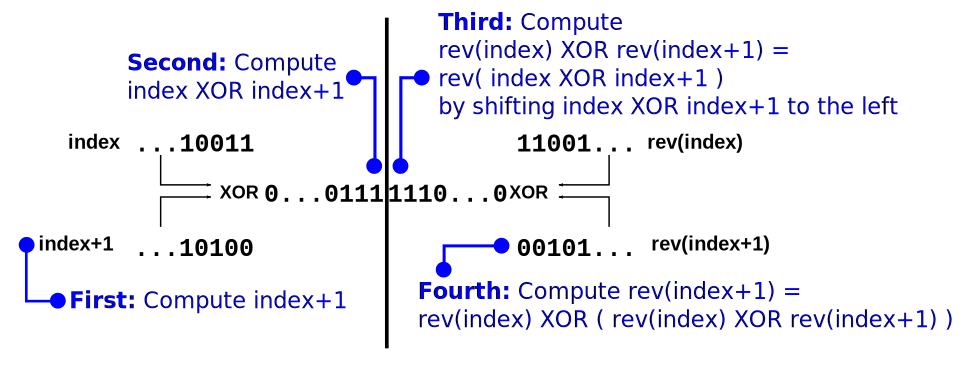
\includegraphics[width=6in]{cartoons/xor.pdf}
\caption{{\bf Illustration der induktiven XOR Methode für das Bit-Reversal} 
    Beginnend mit {\tt index} und seinem reversen Wert 
  {\tt rev(index)}, werden die nächsten Werte ({\tt index+1} und {\tt
  rev(index+1)}) berechnet. Im ersten Schritt wird {\tt index + 1} berechnet. In Schritt 2
  werden die zwischen {\tt index} und {\tt index + 1} verschiedenen Bits mit XOR berechnet. 
  Der resultierende Bitstring hat die Form {\tt 000\ldots 0111\ldots 1}. In Schritt 3 kann 
  dieser dann, wegen seiner besonderen Form, umgekehrt werden, indem er um die Anzahl seiner 
  Nullen nach Links verschoben wird. Im vierten Schritt kann {\tt rev(index + 1)} berechnet werden,
  indem nur noch die verschiedenen Bits mit XOR gekippt werden.
  \label{figure:xor}}
\end{figure}

Die XOR-Mehode ist sehr effizient darin, den nächsten Index und seine Umkehrung zu 
berechnen, erzielt jedoch aus zwei Gründen nur moderate Laufzeiten:
Der Erste ist, dass auf die bitreversen Indizes nicht in cache-optimierter Weise zugegriffen wird. 
%fixme listing
Der zweite Grund ist, dass das {\tt if}-Statement (was auch in {\bf Listing~\ref{alg:simple-permutation}}
zu finden ist) verhindert, dass Loop-Unrolling mit voller Effizienz durchgeführt werden kann, da
zur Compilezeit nicht bekannt ist, welchen Effekt Swapping in einer Iteration auf die folgende Iteration hat, was
die Fähigkeit Swaps parallel auszuführen limitiert. Ebenso sei angemerkt, dass die Häufigkeit, mit der 
sich die Bedingung {\tt index < rev(index)} ändert die Effizienz der Branch-Prediction vermindert.

\paragraph{Unrolling (template-rekursive geschlossene Form):}
%fixme title

Die {\tt if (index < ref(index))} Bedingung zu Eliminieren ist schwierig, da 
das die Vorberechnung der Indizes, auf denen die Bedingung zu {\tt True} evaluiert,
nötig macht, was auffallende Ähnlichkeiten dazu aufweist, das Bit-Reversal selbst zu berechnen.
Allerdings ist es für Probleme von fester Größe (\emph{z.B.}, $b = 10$, bzw. äquivalent dazu $n=1024$)
möglich einfach alle Indizes auf denen Swap ausgeführt werden soll zu berechnen. Das hat zwei Vorteile:
% fixme grammatik
Erstens wird der {\it Overhead} (also die zusätzlichen Kosten, die durch die Codestruktur selbst entstehen) 
von Looping, das Bit-Reversal auf den Indizes auszurechnen und zu Überprüfen, ob {\tt 
index < rev(index)} gilt völlig eliminiert. Zweitens könnte der Compiler theoretisch die Swap-Operationen so anordnen, 
dass die Entfernungsverhältnisse stärker Berücksichtigt werden, also die Cache-Performance optimieren.

Das könnte durch eine hart gecodete Funktion implementiert werden {\tt unrolled\_permutation\_10}, 
oder aber mittels Template-Rekursion zur Compile-Zeit generiert werden. 
Für jeden Bit-String der Form {\tt index = z x y}, wobei {\tt z x y} die Konkatenation der Bit-Strings
{\tt z}, {\tt x} und {\tt y} bezeichnet, ist sein reverses  {\tt rev(index) = rev(y) rev(x)
rev(z)}. Wenn die Bit-Strings {\tt z} und {\tt y} jeweils aus einem einzelnen Bit bestehen, so kann 
ihre Umkehrung ignoriert werden, bzw. ist trivialerweise bereits gegeben: {\tt rev(index) = y rev(x) z}. 
Daher ist es möglich von beiden Enden, also sowohl dem signifikantesten Bit, als auch dem insignifikantesten Bit,
auszugehen und nach innen fortzufahren um rekursiv Probleme der selben Form zu generieren. Die Rekursionsaufrufe
sind dabei mit Template-Rekursion implementiert, werden also bereits zur Compile-Zeit aufgerufen und dienen der
Vorberechnung. Manche der Rekursionsschritte können nach dem Prinzip des Branch-and-Bound abgebrochen werden
({ \bf Abb.~\ref{figure:unrolled}}):
Bitstrings der Form {\tt index = 1~x~0} können nicht kleiner sein, als ihre Umkehrung, egal welchen Wert {\tt x} annimmt. 
Die weitere Rekursion kann abgebrochen werden. Ebenso ist ein Bitstring der Form {\tt index = 0~x~1} immer kleiner als seine 
Umkehrung, und eine Swap-Operation muss für alle möglichen Werte von {\tt x} ausgeführt werden. Bitstrings der Form
{\tt 0~x~0} und {\tt 1~x~1} hingegen werden kleiner als ihre Umkehrung, gdw. {\tt x < rev(x)} gilt. Dieses Problem hat wiederum
die Form des Ausgangsproblems, ist jedoch von geringerer Größe und kann daher rekursiv gelöst werden.

Folglich ist die Laufzeit der Methode durch $r(b) = \underbrace{2^{b-2}}_{gr\ddot un} + \underbrace{2 \cdot
r(b-2)}_{gelb} + \underbrace{0}_{rot}$ gegeben (wobei die angemerkten Farben den Farben in Abb.~\ref{figure:unrolled} entsprechen).
Mit $r(1) = 0$ (für ein einzelnes Bit sind keine Swaps notwendig) und $r(2) = 1$ (für 2 Bits ist genau ein Swap notwendig), folgt die 
geschlossene Form  $r(b) = 2^{\frac{b}{2}} \cdot \left( {(-1)}^b \frac{\sqrt{2}-1}{4} - \frac{1 +
  \sqrt{2}}{4} \right) + 2^{b-1}$. Demzufolge gilt unabhängig davon ob $b$ gerade oder ungerade ist
$r(b) = 2^{b-1} - c \cdot 2^{\frac{b}{2}}$ ($c=\frac{-1}{2}$ wenn $b$ gerade und $c=\frac{-1}{\sqrt{2}}$ wenn 
$b$ ungerade ist). Die asymptotische Laufzeit von dem Term $2^{b-1}$ dominiert und 
daher linear abhängig von $n$ (da $n=2^b$). 

\begin{figure}
\centering
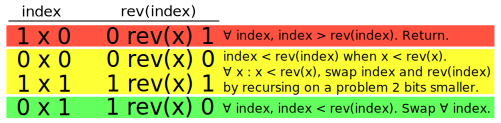
\includegraphics[width=4.5in]{cartoons/unrolled.pdf}
% Fixme
\caption{{\bf Illustration der Unrolled Methode für das Bit-Reversal}
	Alle möglichen Bit-Strings bei denen {\tt index < rev(index)} werden zur Compile-Zeit gefunden, 
	indem mit dem signifikantesten Bit, sowie dem insignifikantesten Bit begonnen wird und nach innen rekursiv 
	vorgegangen wird. Bitstrings der Form {\tt 1~x~0} sind niemals kleiner als ihr reverser Bitstring (in rot hervorgehoben).
	Bitstrings der Form {\tt 0~x~1} sind immer kleiner als ihr reverser Bitstring (in grün hervorgehoben).
	Bitstrings der Form {\tt 0~x~0} und {\tt 1~x~1} sind kleiner als ihr reverser Bitstring, gdw. {\tt x < rev(x)}
	(in gelb hervorgehoben)	
  \label{figure:unrolled}}
\end{figure}

Für kleine Probleme ist diese template-rekursive ``unrolled`` Methode sehr effizient.
Ein Nachteil ist jedoch, dass für große Probleme sehr viel Code generiert wird, was zu hohen 
Kompilierzeiten führt, und bedeuten kann, dass die Ordnung der Swap-Operationen nicht effektiv 
optimiert werden kann. Tatsächlich kann es sein, dass gar keine cache-effiziente Ordnung die 
Indizes aufzurufen existiert, da die reversen Indizes ''herumspringen``. Solange der Compiler also keine 
mathematische Einsicht über die notwendigen Swaps besitzt (was den Compiler dazu befähigen würde, den Code in 
einen der anderen beschriebenen Algorithmen zu transformieren), rechtfertigen die 
mittelmäßigen Laufzeiten auf großen Problemen die substanziellen Kompilierzeiten nicht.

\paragraph{Cache-oblivious rekursive Bit-Reversed Permutation:}
Wenn die Anzahl von Bits $b$ gerade ist, kann ein Index-Bitstring in zwei 
gleich große Teile der Größe $\frac{b}{2}$ partitioniert werden:
{\tt index = x~y}. Der reverse Index ist dann {\tt rev(index)~=~rev(y)~rev(x)}.
Die entsprechende Berechnung kann in drei Schritten durchgeführt werden:
Drehe zuerst die insignifikantesten Bits {\tt y} um {\tt x~rev(y)} zu erhalten. 
Zweitens, swappe die insignifikantesten Bits {\tt y} mit den signifikantesten Bits
% fixme: groß/ klein?
{\tt x} um {\tt rev(y)~x} zu erhalten. Als Drittes, wiederhole den ersten Schritt und drehe 
{\tt x} um {\tt rev(y)~rev(x)~=~rev(index)} zu erhalten.

Dieser rekursive Ansatz ist nicht nur nützlich um einen reversen Index 
zu erzeugen, sondern kann auch dazu benutzt werden die komplette 
Bit-Reversed Permutation rekursiv und lokalisiert durchzuführen, 
sodass der Algorithmus nicht für spezifische Cachegrößen angepasst werden 
muss. Der erste, sowie der dritte Schritt werden auf identische Weise 
durchgeführt: Für alle möglichen signifikantesten Bitstrings führe die
führe eine kleinere, lokalisierte Bit-Reversed Permutation der Größe
$\frac{b}{2}$ aus. Diese rekursive Bit-Reversed Permutation wird vollständig
auf kleineren zusammenhängenden Speicherblöcken ausgeführt und verbessert daher 
die Cacheperformance. Der zweite Schritt, in dem die signifikantesten mit den insignifikantesten
Bits vertauscht werden kann auch als Matrix-Transposition aufgefasst werden, bei der die 
signifikantesten Bits die Reihen der Matrix bilden, und die insignifikantesten die Spalten 
(bei Benutzung von {\tt C}-Style row-order Arrays). Da {\tt x} und {\tt y} durch die gleiche 
Anzahl Bits beschrieben werden, korrespondiert dieser Swap sogar zur Transposition einer quadratischen Matrix,
% fixme cache-oblivious
der in-place ausgeführt werden kann. Weiterhin existiert ein optimaler, cache-olivious Algorithmus
(\emph{d.h.} der Algorithmus operiert in der Nähe optimaler Laufzeiten, 
für jede hierarchische Speicherarchitektur) für die Matrix-Transposition, der diese rekursiv auf kleinere 
Teilprobleme reduziert\cite{prokop:cache}. 
Demnach kann die Bit-Reversed Permutation auf kleinere Bit-Reversed Permutationen auf kleinen 
zusammenhängenden Speicherblöcken und die Transposition einer quadratischen Matrix 
reduziert werden (siehe {\bf Abb.~\ref{figure:recursive}}).

\begin{figure}
\centering
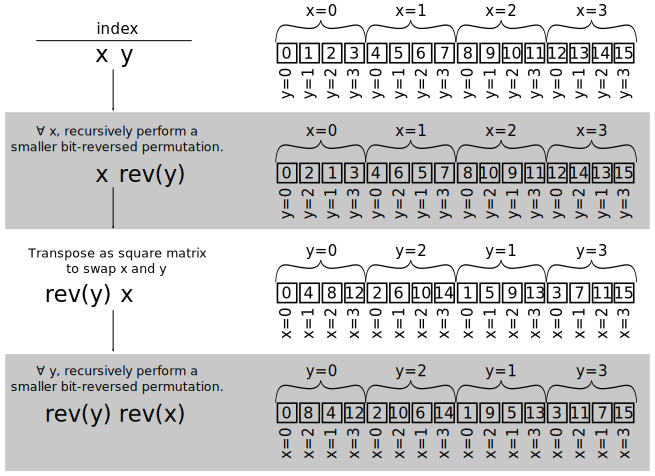
\includegraphics[width=5in]{cartoons/recursive.pdf}
% fixme caption caption
\caption{{\bf Illustration der rekursiven Bit-Reversed Permutation.} 
	Eine Bit-Reversed Permutation auf $b$ bits wird durchgeführt, indem 
	mehrere kleinere Bit-Reversed Permutationen auf $\frac{b}{2}$ Bits,
	eine in-place Transposition einer quadratischen Matrix, sowie weitere kleinere 
	Bit-Reversed Permutationen auf $\frac{b}{2}$ Bits durchgeführt werden. 
	Die Lokalität des Speicherzugriffs in jedem Schritt führt zu einem Cacheeffizienten Algorithmus.
  \label{figure:recursive}}
\end{figure}

Ist die Anzahl der Bits $b$ ungerade, kann zunächst eine einzelne Even-Odd-Permutation
durchgeführt werden: Die Umkehrung von {\tt index = x~y~z}, wobei {\tt z} aus einem 
einzigen Bit besteht, führt zu {\tt rev(index) = z~rev(y)~rev(x)}. Eine Even-Odd-Permutation
erzeugt {\tt z~x~y}. Eine $b-1$ Bit-Reversed Permutation mit {\tt z} = 0 und eine weitere Bit-Reversed 
Permutation {\tt z} = 1 führt zu {\tt z~rev(y)~rev(x)}. Diese Even-Odd-Permutation
im Pre-Processing Schritt führt zu geringfügig höheren Laufzeiten, wenn $b$ ungerade ist. 
Die Even-Odd-Permutation wird out-of-place unter Benutzung eines Buffers der Größe
$\frac{n}{2}$ ausgeführt.

Die Laufzeit der Rekursiven Methode ist durch $r(b) = 2 \cdot 2^{\frac{b}{2}} 
\cdot r(\frac{b}{2}) + 2^b$ definiert. Für diese Rekursionsgleichung existiert eine 
geschlossene Form, gegeben durch  $r(b) = 2^{b-3} \cdot b \cdot c + 2^b \cdot (b-1)$,
wobei $c$ konstant ist. Es gilt also $r(b) \in \Theta(2^b \cdot b) = \Theta(n
\log(n))$.

Trotz der Schwächen der Unrolled-Methode, wenn $b \gg 1$, ist sie sehr effizient 
für kleine und mittelgroße Probleme (\emph{z.B.} $b \leq 14$, was $n \leq 16384$ entspricht)
und daher eine idealer Basisfall (Base-Case) für die Rekursive Methode. Die Rekursionsaufrufe 
können mit Template-Rekursion umgesetzt werden und damit dem Compiler ermöglichen, 
Code zu optimieren, der von den verschiedenen Rekursionsaufrufen 
% fixme groß und klein
gemeinsam genutzt wird. Diese rekursive Methode kann zu einer semi-rekursiven 
Methode generalisiert werden, die die Unrolled-Implementierung nicht nur dann aufruft, 
wenn die Anzahl der Bits niedriger als ein bestimmter Schwellenwert ist,
sondern auch, wenn eine vorher festgelegte Rekursionstiefe überschritten wird. 
Das erlaubt dem Compiler eine stärkere Optimierung, da alle der Template-Rekursiven 
Bit-Reversed Permutationen {\it inline} (\emph{d.h.} der Body der entsprechenden 
Funktion wird im erzeugten Maschinencode direkt an die richtige Stelle geschrieben, 
ohne dass die Funktion extra aufgerufen werden muss, was den Overhead reduziert) 
geschrieben werden können (Bei größeren Rekursionstiefen setzten Compiler nicht immer 
allen Code inline, was man an den viel höheren Kompilierzeiten sehen kann, wenn man die 
Funktion für die rekursive Bit-Reversed Permutation mit {\tt attribute~(\_\_always\_inline\_\_)}
dekoriert, was in  {\tt g++} und {\tt clang} den Compiler zum {\it Inlining} zwingt).
Es sei angemerkt, dass eine semi-rekursive Methode die nur eine einzige Rekursion 
erlaubt eine Laufzeit von  $r(b) = 2 \cdot 2^{\frac{b}{2}} \cdot 2^{\frac{b}{2}} + 2^b$ hat, 
da die rekursiven Aufrufe $r(\frac{b}{2})$ durch die Laufzeit der Unrolled-Methode 
$2^{\frac{b}{2}}$ ersetzt werden. Demzufolge wird die Laufzeit der semi-rekursiven Methode zu 
$2\cdot 2^b + 2^b \in \Theta(2^b) = \Theta(n)$.

Ein Vorteil der rekursiven Methode gegenüber COBRA ist, dass sie komplett in-place, ohne 
einen Buffer ausgeführt werden kann (zumindest, wenn die Anzahl der Bits $b$ gerade ist,
$\frac{b}{2}$ gerade ist, \ldots bis der Basisfall oder die maximale Rekursionstiefe erreicht ist).
Da die rekursive Methode die Bit-Reversed Permutation auf kleinere Bit-Reversed Permutationen und eine 
die Transposition einer Quadratischen Matrix reduziert ist sie gut geeignet für Parallelisierung mit SIMD, 
Multicore-CPUs oder GPUs; Parallelisierung von COBRA würde einen zusätzlichen Buffer für jeden Thread 
erfordern um {\it Race-Conditions} zu vermeiden.\newline

Die asymptotischen Laufzeiten aller Methoden sind in {\bf Tabelle~\ref{table:theoretical-runtimes}} aufgelistet.

\begin{table}[ht!]
  \centering
  \small
  \scalebox{0.88}{
    \begin{tabular}{c|cccccccc}
      & Stockham & Bitwise & Bytewise & Pair bitwise & COBRA & Unrolled & XOR & Recursive \\
      \hline
      %& \multicolumn{3}{c}{$d$ known at compile time} \\
	  {\bf Runtime} & \multirow{2}{*}{$n \log(n)$} & \multirow{2}{*}{$n \log(n)$} & \multirow{2}{*}{$n \log(n)$} & \multirow{2}{*}{$n \log(n)$} & \multirow{2}{*}{$n + \frac{n}{t} \log(\frac{n}{t})$} & \multirow{2}{*}{$n$} & $n$ or & $n$ or \\ 
          (asymptotic) & & & & & & & $n \log(\log(n))$ & $n \log(n)$\\
	  \hline
    \end{tabular}
  }
  \caption{{\bf Theoretische Laufzeiten.} 
      Für jeden der beschriebenen Algorithmen sind die asymptotischen Laufzeiten aufgeführt. 
    Es sei angemerkt, dass die Algorithmen mit der niedrigsten theoretischen Laufzeit nicht unbedingt 
    auch in der Praxis schneller sind: Beispielsweise sind sowohl die Bitwise- wie auch die Bytewise-Methode
    $\in \Theta(n\log(n))$, jedoch hat die Bytewise-Methode eine bessere Laufzeitkonstante, da sie eine Tabelle nutzt um 
    Wörter der Länge 8 Bit auf einmal umzukehren. Auch greifen die Pair-Bitwise Methode, COBRA, sowie die rekursiven Methoden
    in lokalerer Art und Weise auf den Cache zu, haben also eine größere Cache-Lokalität. Im Term der COBRA Methode
    bezeichnet $t$ die Größe des Buffers. Die Laufzeit der induktiven XOR Methode ist entweder $\in \Theta(n)$ (wenn die 
    Methode um die Anzahl der führenden Nullen zu zählen in $\Theta(1)$ ist) oder $\in \Theta(n \log(\log(n)))$ (wenn das Zählen der 
    Nullen nicht Hardwareseitig unterstützt wird, und daher $\in \Theta(\log(\log(n)))$ Schritte benötigt). Die
    rekursive Methode benötigt i.A. $\in \Theta(n \log(n))$ Schritte, kann aber beschleunigt werden auf $\in \Theta(n)$ Schritte,
    wenn ein semi-rekursiver Ansatz, der die Rekursionstiefe begrenzt, verfolgt wird. 
    }
  \label{table:theoretical-runtimes}
\end{table}

\section*{Results}
Alle Methoden wurden in {\tt C++11} implementiert und machen von Template-Rekursion 
und {\tt constexpr} Variablen und Funktionen gebrauch. Die Laufzeiten wurden verglichen, indem für alle Methoden
% fixme Kompilieren, Compiler
Benchmarks durchgeführt wurden, die sowohl mit {\tt clang++ 3.8.0} als auch {\tt g++ 6.2.0} kompiliert wurden.
Bei beiden Compiler wurde die Optimierung durch die Flags {\tt -Ofast -march=nativ -mtune=native} genutzt. 
Um kein Pointer Aliasing oder andere Interferenzen zwischen den einzelnen Benchmarks zu riskieren wurde für jeden Algorithmus
und jede Problemgröße eine seperate {\tt main.cpp} Datei erzeugt. Kompilierzeiten mit 
{\tt clang++} sind in {\bf
  Abb.~\ref{fig:clang++_compile_times}} dargestellt, Kompilierzeiten mit {\tt g++}
in {\bf Abb.~\ref{fig:g++_compile_times}}. Alle Methoden wurden auf Arrays von Typ
{\tt std::complex<double>} angewandt, da unsere primäre Motivation darin bestand, die Eignung der Methoden für die FFT zu evaluieren.
Man beachte, dass die tatsächlichen Laufzeiten schwanken können wenn andere Datentypen wie {\tt int} oder {\tt float} genutzt werden.
Für die in-place und die out-of-place COBRA Methoden wurden die Buffer-Größen für jede Problemgröße optimiert.
Die cache-oblivious rekursive Methode verwendet einen Basisfall der Größe $b \leq 9$, verwendet also die geschlossene Form 
% fixme split sentences
der Unrolled-Methode für entsprechende Problemgrößen. Die Abhängigkeit der Laufzeit von der Größe des Basisfalls war 
nicht sehr stark, was Ähnlichkeiten mit der Größe des Basisfalls bei der cache-oblivious Matrix-Transposition aufweist, wo dieser nur 
dazu verwendet wird, die Kosten der Rekursion zu Amortisieren, indem sicher gestellt wird, dass die Berechnungskosten des Basisfalls nicht 
trivial werden.

Die Problemgrößen der Benchmarks reichten von $n=2^8$ (was ca. $4$ KB Speicherplatz benötigt) bis $n=2^{30}$
(was ca. $16.4$ GB Speicherplatz benötigt). Für alle Messungen wurde der Durchschnitt über 100 Wiederholungen gebildet. 
Die Ergebnisse sind als Lauzeiten pro Element, \emph{d.h.} die Laufzeit der kompletten Bit-Reversed Permutation, 
geteilt durch die Anzahl der Elemente $n$, notiert. Die CPU-Spezifikation des verwendeten Testsystems 
ist in {\bf Tabelle~\ref{table:cpu_spec}} aufgeführt. Die Laufzeiten aller Tests sind in {\bf Abb.~\ref{fig:clang++_runtimes}} 
für {\tt clang++} und in {\bf Abb.~\ref{fig:g++_runtimes}} für {\tt g++} aufgeführt.

Um die Parallelisierbarkeit der semi-rekursiven Methode zu testen wurden parallele Versionen implementiert und verglichen:
% fixme Oliver nerven!
Die erste wurde mit OpenMP und der {\tt -fopenmp} Compiler-Option umgesetzt. Diese Implementierung nutzt 
{\tt \#pragma omp parallel for} um die Rekursionsaufrufe (die die geschlossene Form der Unrolled-Methode aufrufen, 
da nur ein Rekursionsschritt erlaubt ist) zu parallelisieren. Die zweite Version nutzt das CUDA-Toolkit um die semi-rekursive Methode 
auf der GPU zu parallelisieren. Die CPU-Version erlaubt zwei Rekursionen und ist fest für $b=24$ implementiert 
(es ist notwendig, die Indizes in einem Array zwischenzuspeichern, welches dann auf die GPU übertragen wird).
$b=24$ wurde gewählt, weil $b=24$ durch 4 Teilbar ist und dem größten Array entspricht, welches noch komplett auf die GPU passt
(Problemgrößen, die durch 4 Teilbar sind, können 2 Rekursionsschritte durchlaufen, ohne dass eine Even-Odd-Permutation notwendig wird).
Die CUDA-Implementierung führt in-place Matrix-Transpositionen auf der GPU aus\cite{harris:cuda}, parallelisiert also sowohl 
die Rekursion, als auch die Matrix-Transposition (das hat den zusätzlichen Vorteil, dass die Daten nur 
einmal auf die GPU übertragen werden müssen). Die OpenMP Version und die CUDA version wurden mit {\tt g++} (CUDA nutzt zusätzlich {\tt nvcc})
kompiliert, da {\tt clang++} derzeit keine Unterstützung für OpenMP oder CUDA bietet. Die parallelisierten Versionen werden in 
{\bf Abb.~\ref{fig:g++_parallel_runtimes}} mit den am besten abschneidenden Single-Thread Versionen verglichen.


\begin{table}[ht!]
  \centering
  \begin{tabular}{cccccc} L1d &  L1i &    L2 &      L3 & MAX\_SPEED &   RAM \\
\midrule
 32K &  32K &  256K &  15360K &    3.8Ghz &  65GB \\
\end{tabular}
\caption{ {\bf CPU-Spezifikation des Benchmarking-Systems} 
    Die Größe des L1 Data-Caches, des L1 Instruction-Caches, des L2 und L3 Caches,
    die maximale CPU-Taktfrequenz sowie die Größe des RAMs des Computers der für 
    die Tests genutzt wurde sind aufgelistet. Um diese Angaben in Relation zu den 
    Benchmark-Ergebnissen zu setzen, sei angemerkt, dass $32$K ein Array von  
    $n=2^{11}$ Elementen vom Typ {\tt std::complex<double>} speichern können. 
    Entsprechend können $256$K $n=2^{14}$ Elemente und $15360$ K $n=2^{20}$ Elemente speichern.
    In den RAM von $65$GB passen $n=2^{31}$ Elemente. 
    \label{table:cpu_spec}
}
\end{table}

\begin{figure}[ht!]
\centering
  \includegraphics[width=4.5in]{results/clang++_compile_times.pdf}
\caption{{\bf Kompilierzeiten mit {\tt clang++}}. 
    Dargestellt sind die Kompilierzeiten für jede Methode in Abhängigkeit der Problemgrößen.
    Die $t$-Achse ist logarithmisch skaliert. Die entsprechenden Laufzeiten sind in 
    %fixme: -> Guter Name; UnrolledShuffle
    {\bf Abb.~\ref{fig:clang++_runtimes}} dargestellt. Die UnrolledShuffle Methode wurde 
    für Problemgrößen $b>16$ nicht mehr kompiliert, da die Größen der ausführbaren Dateien, 
    wie auch die Kompilierzeiten nicht mehr sinnvoll wären.
    \label{fig:clang++_compile_times}	
}
\end{figure}

\begin{figure}[ht!]
\centering
  \includegraphics[width=4.5in]{results/g++_compile_times.pdf}
\caption{{\bf Kompilierzeiten mit {\tt g++}}. 
    Dargestellt sind die Kompilierzeiten für jede Methode in Abhängigkeit der Problemgrößen.
    Die $t$-Achse ist logarithmisch skaliert. Die entsprechenden Laufzeiten sind in 
    {\bf Abb.~\ref{fig:g++_runtimes}} dargestellt. Die UnrolledShuffle Methode wurde 
    für Problemgrößen $b>16$ nicht mehr kompiliert, da die Größen der ausführbaren Dateien, 
    wie auch die Kompilierzeiten nicht mehr sinnvoll wären.
    \label{fig:g++_compile_times}	
}
\end{figure}

\begin{figure}[ht!]
\centering
  \includegraphics[width=6in]{results/clang++_run_times.pdf}
\caption{{\bf Laufzeiten pro Element mit {\tt clang++}}. 
    Dargestellt sind die Laufzeiten pro Element der Bit-Reversed Permutation für 
    jede Methode und jede Problemgröße. Die Laufzeiten sind über $100$ Durchläufe gemittelt
    und wurden Anschließend durch die Anzahl der Elemente (\emph{d.h.} $n=2^b$) geteilt.
    Die farbigen Bereiche stellen die minimalen, bzw. die maximalen Laufzeiten der 100 Wiederholungen dar.
    Der linken Seite sind alle getesteten Problemgrößen von $b=4$ bis $b=31$ dargestellt. Auf der 
    rechten Seite sind nur die Laufzeiten der Methoden die am besten Abschneiden auf den größeren Problemen von
    $b=20$ bis $b=30$ dargestellt. Die Methoden mit schlechter Laufzeit (Stockham, Bitwise, Bytewise und XOR) wurden
    für $b>26$ von den Tests ausgeschlossen.
  \label{fig:clang++_runtimes}	
}
\end{figure}

\begin{figure}[ht!]
\centering
  \includegraphics[width=6in]{results/g++_run_times.pdf}
\caption{{\bf Laufzeiten pro Element mit {\tt g++}}. 
    Dargestellt sind die Laufzeiten pro Element der Bit-Reversed Permutation für 
    jede Methode und jede Problemgröße. Die Laufzeiten sind über $100$ Durchläufe gemittelt
    und wurden Anschließend durch die Anzahl der Elemente (\emph{d.h.} $n=2^b$) geteilt.
    Die farbigen Bereiche stellen die minimalen, bzw. die maximalen Laufzeiten der 100 Wiederholungen dar.
    Der linken Seite sind alle getesteten Problemgrößen von $b=4$ bis $b=31$ dargestellt. Auf der 
    rechten Seite sind nur die Laufzeiten der Methoden die am besten Abschneiden auf den größeren Problemen von
    $b=20$ bis $b=30$ dargestellt. Die Methoden mit schlechter Laufzeit (Stockham, Bitwise, Bytewise und XOR) wurden
    für $b>26$ von den Tests ausgeschlossen.
  \label{fig:g++_runtimes}	
}
\end{figure}


\begin{figure}[ht!]
\centering
  \includegraphics[width=6in]{results/open_mp_performance.pdf}
\caption{{\bf Performancegewinn durch Parallelisierung}. Die Benchmarks 
    aus {\bf Abb.~\ref{fig:g++_runtimes}} sind erneut dargestellt, jedoch unter Einschluss
    der parallelisierten Versionen der semi-rekursiven Methode. Durch ihre inhärente
    Parallelisierbarkeit resultiert OpenMP leicht in größerer Performance. 
    Parallelisierung auf der GPU mit CUDA erreicht sogar noch bessere Parallelität.  
  \label{fig:g++_parallel_runtimes}
}
\end{figure}

\section*{Discussion}
Sowohl mit {\tt g++} als auch {\tt clang++} haben die Stockham und die naive Bit-Wise Methode 
ähnlich abgeschnitten. Es handelt sich um die Ineffektivsten der hier untersuchten Methoden.
Die Stockham Methode funktioniert out-of-place (was die Cache-Last erhöht) und führt mehr Swaps 
durch als die naive Bitwise Methode, greift aber auf die Elemente geteilt nach geraden und ungeraden Indizes zu,
hat also eine bessere Cache-Lokalität, wohingegen die Bit-Wise Methode auf die Daten in einem weniger 
zusammenhängenden Muster zugreift, da in jeder Iteration auf {\tt rev(i)} zugegriffen wird.

Die Bytewise Methode und die XOR Methode schneiden ähnlich ab. Beide Methoden skalieren 
bedeutend besser als die Stockham oder die Bitwise Methode. Beide erreichen ein schnelleres Bit-Reversal, 
jedoch nutzt keine der beiden ein zusammenhängendes Speicherzugriffsmuster. Die XOR Methode könnte dennoch 
ihre Anwendungsgebiete in Gebieten, in denen Speicher sehr kostbar ist (\emph{z.B.} eingebettete Systeme) haben,
da sie ähnliche Leistung wie die Bytewise Methode erreicht, jedoch ohne eine Tabelle von $256$B zu benötigen. 

Betrachtet man den Fall, dass das komplette Array in den L1 Cache passt, erreicht die Unrolled-Methode im Grunde 
optimale Leistung, da kein Overhead für Schleifen, Bit-Reversal oder bedingte Anweisungen generiert wird. 
Außerdem können die Operationen so kompiliert werden, dass sie unmittelbare Addressierung im Assembly-Code verwendenden,
die Indizes also nativ in den Assembly-Code selbst geschrieben werden und nicht in einem seperaten Array gespeichert werden müssen.
Der Laufzeitvorteil gilt jedoch nicht für große Probleme (wenn das Array nicht in den L1 oder L2 Cache passt) und auch die Kompilierzeiten 
werden sehr groß (ca. 100 Sekunden wenn $n=16$, sowohl für {\tt clang++} als auch für {\tt g++}).

Die leistungsfähigsten Algorithmen auf großen Problemen sind die, die für die der Cache berücksichtigt wurde: Das schließt die 
Pair-Bitwise Methode, COBRA (sowohl in-place, als auch out-of-place) und die rekursive Methode, bzw. ihre semi-rekursive Variante ein.
Die rekursive und die semi-rekursive Methode profitieren von geraden Problemgrößen, da in diesem Fall keine Even-Odd Permutation durchgeführt werden muss (was zu dem Sägezahn-Muster in den Laufzeiten auf großen Problemen führt). Die semi-rekursive Variante erreicht geringfügig bessere
Performance, was jedoch mit einer erhöhten Kompilierzeit (zwischen 10 und 13 Sekunden für $b=28$) bezahlt werden muss. 
Für kleinere Probleme ist die out-of-place COBRA Methode weniger effizient als ihre in-place Variante, da der Cache durch den doppelten 
Speicherverbrauch stärker belastet wird. Auf größeren Problemen wird jedoch durch die out-of-place Variante die größere Leistung gebracht,
da die out-of-place Variante die Werte mithilfe eines Buffers kopiert, während die in-place-variante den Buffer für Swaps nutzt, und daher 
in den Buffer kopieren, anschließend den Swap zwischen Buffer und Array durchführen und anschließend die 
resultierenden Änderungen der Werte wiederum in das Array zurückschreiben muss.

Die Pair-Bitwise Methode führt zwar  mehr Swap-Operationen aus, diese jedoch in einem zusammenhängenderen Zugriffsmuster 
und ohne die Nutzung eines zusätzlichen Buffers. Die Pair-Bitwise Methode, die COBRA Methoden und die rekursive bzw. semi-rekursive Methode
schneiden auf großen Problemen ähnlich ab; die out-of-place COBRA Methode funktioniert am besten, verliert jedoch ihren Vorsprung, wenn die 
Buffer-Größe nicht für die spezifische CPU optimiert wird. 
Es sind kleine Anstiege in der Laufzeit pro Element zu beobachten, am stärksten sichtbar an der L3-Cache Grenze bei $b=18$ für
die in-place Methoden und $b=17$ für die out-of-place Methoden. 

Im Gegensatz zu den COBRA Methoden, die einen Matrix-Buffer nutzen um hohe Leistung zu erreichen, sind die rekursive 
und semi-rekursive Methode inhärent cacheeffizient und benötigen keinen Buffer, was sie gut geeignet für eine Parallelisierung macht.
{\bf Abb.~\ref{fig:g++_parallel_runtimes}} zeigt den starken Performancezuwachs, den grober Paralellismus mit OpenMP oder 
feingranularer Parallelismus mit CUDA, bringen kann. Die Rekursionen benötigen keinerlei Informationen von anderen Elementen und sind daher
perfekt für nebenläufige Verarbeitung geeignet; auch auf modernen CPUs, die Teilweise separate L1-Caches für jeden Kern mitbringen.
Es ist sehr wahrscheinlich, dass die inhärente Parallelisierbarkeit auch noch stärker für eine hoch optimierte CUDA Implementierung 
ausgenutzt werden kann.

Bei $b=24$ benötigt die schnellste nicht-parallele Methode knapp weniger als $8 \times {10}^{-9}$ Sekunden pro Element, bzw. 0.13 Sekunden
für die komplette Prozedur. Im Vergleich dazu benötigt die OpenMP Variante $0.1$ Sekunden, die GPU Variante sogar nur $0.8$ Sekunden. 
Die {\tt numpy} FFT (die die {\tt FFTPACK}-Library benutzt) benötigt rund $2$ Sekunden für ein Problem dieser Größe. Naives Bit-Reversal benötigt
ca. $1$ Sekunde, was darauf schließen lässt, dass ca. 50 \% der kompletten Laufzeit mit der Bit-Reversed Permutation verbracht wird. 
Obwohl der Butterfly-Code der FFT kompliziertere Manipulationen komplexer Zahlen durchführt, geschieht das in 
zusammenhängenden Speicherzugriffsmustern, was wiederum die Bit-Reversed Permutation wichtiger macht, als es zunächst scheint.
Weiterhin würde der Ansatz, die semi-rekursive Methode zu nutzen um die volle FFT auf der GPU durchzuführen nicht nur davon profitieren, die kleinen
Butterfly-Operationen parallel durchzuführen, sondern auch die Laufzeit der Bit-Reversed Permutation substanziell senken, indem vermieden wird,
die Daten auf die GPU zu kopieren, bzw. sie am Ende wieder von der GPU runter zu holen.

Neben der Eigenschaft der Parallelisierbarkeit der rekursiven Methoden kommt ihr Vorteil auch daher, dass sie eine hohe Leistung erreichen, ohne 
für spezifische Cache-Architekturen optimiert werden zu müssen (was einen starken Einfluss auf die Leistung der COBRA Methoden hat). 
Die rekursive Methode ist cache-oblivious. Wenn sie mit einer optimalen cache-oblivious Methode für die Matrix-Transposition 
\cite{prokop:cache}gekoppelt wird, garantiert sie ein einigermaßen zusammenhängendes 
Speicherzugriffsmuster ohne zusätzliche Informationen über die Cache-Architektur.
Wie auch die rekursive Methode, braucht die semi-rekursive Methode keinen Buffer mit einer für die Cache-Architektur optimierten Größe.
Dennoch ist die semi-rekursive Methode nicht cache-oblivious, da es sein kann dass ein großes Problem nicht auf Probleme, die komplett in den Cache 
passen, reduziert wird. Die rekursive Methode ist nicht nur für Untersuchungen über Leistungssteigerung durch 
Parallelisierung interessant, sondern könnte auch ein vielversprechender Startpunkt für die Suche nach einem optimalen 
Algorithmus für die Bit-Reversed Permuation sein.

\section*{Availability}
Sämtlicher beiliegender {\tt C++11} Quellcode, die vorläufige GPU Implementierung 
des rekursiven Algorithmus, Benchmarking Scripts, sowie der \LaTeX\ Code für das Paper selbst
sind frei verfügbar (Creative Commons Lizenz) unter 
\url{https://bitbucket.org/orserang/bit-reversal-methods}.\newline

\section*{Danksagungen}

Wir bedanken uns bei Thimo Wellner und Guy Ling für deren Beiträge. \newline

\noindent Dieses Paper wurde als Teil des Master-Kurses {\it Scientific Computing} 
im Wintersemester 2016--2017 an der Freien Universität Berlin, gelehrt von Oliver Serang,
geschrieben. Übersetzungen dieses Papers sind auf Englisch und in den Muttersprachen der Studenten
Deutsch, Chinesisch, Türkisch und Spanisch verfügbar. 

\section*{Beiträge der einzelnen Autoren}
Das Projekt wurde geleitet von O.S., der ebenso die neuen Algorithmen entwickelt und die nicht parallelen 
Versionen der getesten Algorithmen in {\tt C++11} implementiert hat. Die Einleitung wurde von X.W. verfasst.
Der Methodenteil und die Laufzeitanalyse stammen von B.A., X.W. und D.W. Die OpenMP Implementierung wurde von O.S. geschrieben, 
die GPU Variante von B.A. Die Benchmarks, Abbildungen, sowie der Ergebnisteil wurde von C.K. verfasst. Der Diskussionsteil stammt von 
X.W. und C.K. Tests und optimierung wurden von B.A. und D.W. durchgeführt. Die abschließenden Benchmarks wurden von C.K., L.I., T.C. und O.S.
durchgeführt. \newline
\noindent Die Seniorautoren (O.S. und T.C.) ausgeschlossen wurde die Reihenfolge der Autoren in einer geheimen Abstimmung 
von den Studenten festgelegt. 

% bibliography:
\bibliographystyle{unsrt}
\bibliography{refs.bib}


\end{document}

